\documentclass[11pt]{article}

% Geometry and margins
\usepackage[margin=1in]{geometry}

% Hyperlinks
\usepackage{hyperref}

% Mathematics
\usepackage{amsmath}
\usepackage{amssymb}

% Tables
\usepackage{booktabs}

% Graphics
\usepackage{graphicx}

% Colors
\usepackage{xcolor}

% Code listings
\usepackage{listings}
\lstset{
  basicstyle=\footnotesize\ttfamily,
  breaklines=true,
  breakatwhitespace=true,
  columns=flexible,
  keepspaces=true,
  showstringspaces=false,
  frame=single,
  framesep=4pt,
  xleftmargin=6pt,
  xrightmargin=6pt,
}

% Bibliography
\usepackage{natbib}

% -------------------------------------------------------

\title{Infon: A Knowledge Graph Reasoner with Calibrated Uncertainty}

\author{
  Eden Duthie \\
  Trusst.ai \& AgenticX \\
  \texttt{eduthie@trusst.ai} \\
  \texttt{eduthie@agenticx.org}
  \and
  Charles Prosper \\
  Amazon Web Services
  \and
  Josh Passenger \\
  Amazon Web Services
}

\date{May 2026}

% -------------------------------------------------------

\begin{document}

\maketitle

\begin{abstract}
Infon is a knowledge graph reasoner that performs fact-checking over
document corpora with calibrated uncertainty. Three properties distinguish it
from prior systems: \emph{cassette-native storage} (immutable,
content-addressed, S3-native documents with manifest pruning), \emph{honest
uncertainty} via a first-class Dempster--Shafer vacuous element~$m(\Theta)$
that rises to $1.0$ on unsupported claims rather than fabricating confident
answers, and \emph{MCTS multi-hop reasoning} guided by a frozen sheaf graph
neural network as a terminal scorer. On the actor-to-actor real-data
evaluation, the symbolic pipeline scores $80\%$ accuracy; adding the sheaf
GNN raises this to $100\%$. On synthetic held-out data the GNN reaches
$99.2\%$ overall accuracy. The system operates on a laptop CPU without GPU or
API keys. Code is released under the repository tag \texttt{v0.4.0-paper}.

\end{abstract}

\section{Introduction}
\label{sec:introduction}

Fact-checking over document corpora is a central task in applied NLP: given a
claim and a collection of source documents, a system must decide whether the
corpus supports the claim, refutes it, or provides no relevant evidence.
Current approaches fall into two failure modes. Retrieval-augmented generation
(RAG) systems retrieve supporting passages and feed them to a language model,
which can \emph{hallucinate} verdicts on claims the corpus does not speak
to~\cite{lewis2020rag}. Knowledge-graph pipelines that extract structured
triples achieve better grounding but require rigid, hand-curated schemas and
cannot express that a question simply lacks an answer in the available
evidence~\cite{hogan2021kg}.

Neither class of system handles \emph{multi-hop} reasoning with
\emph{calibrated uncertainty}: the ability to chain intermediate facts across
documents while simultaneously signalling when the chain is absent or
incomplete. This gap is consequential. A compliance analyst who asks whether
company A indirectly supplies component B via an intermediate supplier needs
both the chain and an honest ``the corpus does not say'' when the chain is
missing.

\paragraph{This paper.}
We present \textbf{Infon}, a deployable knowledge graph reasoner that
fills this gap. Infon is not a neural language model; it is a symbolic
reasoner augmented by a learned prior. Its design is guided by five
engineering properties:

\begin{enumerate}
  \item \textbf{Cassette-native storage.}  Documents are stored as immutable,
    content-addressed \texttt{.inf} files that can live on S3 or a local
    filesystem via \texttt{fsspec}. Delta ingests append; nothing is rewritten.
    A manifest pruner skips cassettes that cannot contain the query anchor,
    cutting Parquet opens by 7--16$\times$ at scale and 278$\times$ on cache
    misses.

  \item \textbf{Schema-free operation.}  Plain-English questions are encoded
    with SPLADE-tiny~\cite{formal2021splade} (17~MB, Apache~2.0, no GPU)
    to an anchor vocabulary. Connective predicates are auto-inferred from the
    data: no ontology annotation is required. A Strands-powered \texttt{Analyst}
    agent routes natural-language questions to the appropriate retrieval
    primitive, citing every source it uses.

  \item \textbf{Dempster--Shafer mass with first-class} $\boldsymbol{m(\Theta)}$.
    Every verdict is a four-part mass $(m_S, m_R, m_U, m_\Theta)$ over the
    frame $\Omega = \{S, R, U\}$ (Supports, Refutes, Uncertain), where
    $m_\Theta = m(\Omega)$ is the vacuous element that rises to $1.0$ on
    unsupported claims rather than a confident wrong answer~\cite{shafer1976mathematical}.

  \item \textbf{MCTS and sheaf GNN multi-hop reasoning.}  A Monte Carlo Tree
    Search traverses the infon hypergraph, with a 140k-parameter frozen sheaf
    graph neural network~\cite{bodnar2022sheaf} serving as the terminal scorer.
    The GNN provides the MCTS prior that guides search toward high-confidence
    chains.

  \item \textbf{Schema evolution without reingestion.}  A categorical
    \texttt{SchemaFunctor} rewrites existing cassettes under a new ontology
    via a Kan pushforward. Old snapshots remain queryable; the migration is
    62$\times$ faster than re-extraction.
\end{enumerate}

\paragraph{Roadmap.}
Section~\ref{sec:background} establishes the formal background: Dempster--Shafer
theory, situation semantics and infons, SPLADE sparse retrieval, and sheaf
graph neural networks.
Section~\ref{sec:architecture} describes Infon's four-layer architecture
(cassette substrate, query DSL, reasoner, and conversational analyst).
Section~\ref{sec:implementation} details the implementation, including the
synthgen corpus, GNN training, and manifest pruner benchmarks.
Section~\ref{sec:experiments} reports experimental results on synthetic and
real-world evaluations (HoVer~\cite{jiang2020hover},
AVeriTeC~\cite{schlichtkrull2023averitec},
SciFact~\cite{wadden2020scifact}).
Section~\ref{sec:discussion} discusses limitations and future work.
Section~\ref{sec:related_work} surveys related work.
Section~\ref{sec:conclusion} concludes.
Section~\ref{sec:reproducibility} provides a system card and reproducibility
statement.

\section{Background}
\label{sec:background}

This section establishes notation and reviews the four theoretical foundations
that Infon builds on.

% -----------------------------------------------------------------------
\subsection{Dempster--Shafer Theory}
\label{sec:background:ds}

Dempster--Shafer (DS) theory~\cite{dempster1967upper,shafer1976mathematical}
generalises Bayesian probability by allowing belief to be assigned to
\emph{sets} of hypotheses rather than individual hypotheses, thereby
distinguishing \emph{uncertainty} (evidence spread over possibilities) from
\emph{ignorance} (absence of evidence).

\paragraph{Frame of discernment.}
Let $\Omega$ be a finite, mutually exclusive, exhaustive set of hypotheses
called the \emph{frame of discernment}.  Infon uses
\[
  \Omega = \{S,\, R,\, U\},
\]
where $S$ = Supports, $R$ = Refutes, and $U$ = Uncertain/mixed.

\paragraph{Basic probability assignment.}
A \emph{basic probability assignment} (bpa) is a function
$m \colon 2^{\Omega} \to [0,1]$ satisfying
\[
  m(\emptyset) = 0 \qquad \text{and} \qquad \sum_{A \subseteq \Omega} m(A) = 1.
\]
Each focal element $A$ with $m(A) > 0$ represents a portion of belief
committed to ``the truth lies somewhere in $A$'' without further
discrimination.

\paragraph{Vacuous element.}
The \emph{vacuous} bpa commits all mass to the full frame:
\[
  m(\Theta) = 1, \quad m(A) = 0 \text{ for all } A \subsetneq \Omega.
\]
Here $\Theta$ denotes $\Omega$ itself when used as a focal element; the
notation $m(\Theta)$ refers to the mass on this total-ignorance element.
It is the \emph{correct} encoding for ``No Evidence Identified'' (NEI): it
expresses that the available evidence does not constrain the hypothesis at all,
as opposed to $m(U) > 0$, which would assert that conflicting evidence
\emph{was} observed.

\paragraph{Dempster's combination rule.}
Given two independent bpas $m_1$ and $m_2$ over the same frame, their
\emph{orthogonal sum} $m = m_1 \oplus m_2$ is defined for all $A \neq
\emptyset$ as
\[
  m(A) = \frac{1}{1 - K} \sum_{\substack{B \cap C = A \\ B,\,C \subseteq \Omega}} m_1(B)\, m_2(C),
\]
where the normalisation constant $K = \sum_{B \cap C = \emptyset} m_1(B)\, m_2(C)$
accounts for conflicting evidence.  Combination is commutative and associative,
so evidence from multiple infons can be fused incrementally.

\paragraph{Four-part mass in Infon.}
Throughout this paper, a verdict mass is written as the tuple
$(m_S,\, m_R,\, m_U,\, m_\Theta)$, where
\[
  m_S = m(\{S\}), \quad
  m_R = m(\{R\}), \quad
  m_U = m(\{U\}), \quad
  m_\Theta = m(\Theta),
\]
and $m_S + m_R + m_U + m_\Theta = 1$.
An \emph{unsupported} claim has $m_\Theta \approx 1$ (no focal evidence);
a \emph{supported} claim has $m_S \approx 1$; a \emph{refuted} claim has
$m_R \approx 1$.  The chain-mass accumulation and GNN scoring described in
Sections~\ref{sec:architecture} and~\ref{sec:implementation} produce masses
in this form.

% -----------------------------------------------------------------------
\subsection{Situation Semantics and Infons}
\label{sec:background:infons}

Infon's unit of extracted knowledge is the \emph{infon}, drawn from
Barwise and Perry's situation semantics~\cite{barwise1983situations}.

\paragraph{Infon triple.}
An infon is a typed quadruple
\[
  \langle\!\langle \mathit{pred},\; \mathit{subj},\; \mathit{obj};\; \mathit{pol} \rangle\!\rangle,
\]
where $\mathit{pred}$ is a predicate label, $\mathit{subj}$ and $\mathit{obj}$
are entity anchors, and $\mathit{pol} \in \{+1, -1\}$ records whether the
predicate holds ($+1$, affirmed) or is negated ($-1$).

\paragraph{Grounding.}
Each infon is grounded to its source: a \emph{cassette} identifier (the SHA-256
content hash of the document), a byte \emph{offset} into the cassette's record
stream, and an extraction \emph{timestamp}.  This grounding lets Infon cite
the exact passage that generated each mass contribution and supports
time-travel queries over snapshot manifests.

\paragraph{Why infons?}
Infons are the natural unit for two reasons.  First, their polarity field
directly encodes negation, so refuting evidence is represented symmetrically
with supporting evidence.  Second, the triple structure $(\mathit{pred},
\mathit{subj}, \mathit{obj})$ maps cleanly onto a hypergraph edge, enabling
MCTS traversal along predicate-typed chains.

% -----------------------------------------------------------------------
\subsection{SPLADE Sparse Retrieval}
\label{sec:background:splade}

SPLADE~\cite{formal2021splade} (Sparse Lexical and Expansion model) trains a
BERT-family encoder to produce high-dimensional \emph{sparse} activations over
a fixed vocabulary.  For a text sequence $t$, the SPLADE encoder produces a
vector $\mathbf{s} \in \mathbb{R}^{|\mathcal{V}|}$ whose $k$-th component is
\[
  s_k = \log\!\bigl(1 + \mathrm{ReLU}(h_k)\bigr),
\]
where $h_k$ is the aggregated BERT hidden state for vocabulary token $k$.
Only a small fraction of dimensions are non-zero, so $\mathbf{s}$ can be
stored and intersected efficiently with an inverted index.

\paragraph{SPLADE-tiny in Infon.}
Infon uses the \texttt{naver/splade-v3-lexical} distilled variant
(17~MB, Apache~2.0 licence).  It runs on CPU in under 2~seconds cold-start
and requires no GPU or external API.  Each ingested document is encoded into a
sparse anchor vector; at query time, the query anchor is matched against
cassette-level bounding boxes in the manifest pruner, and the top-scoring
cassettes are hydrated for full scoring.  This design keeps retrieval
complexity proportional to the number of \emph{relevant} cassettes rather than
the total corpus size.

% -----------------------------------------------------------------------
\subsection{Sheaf Graph Neural Networks}
\label{sec:background:sheaf_gnn}

A sheaf graph neural network~\cite{bodnar2022sheaf} augments a standard message-passing
GNN with \emph{restriction maps}: for each edge $(u, v)$ in the graph, a
learnable linear map $F_{u \trianglelefteq e} \colon \mathbb{R}^d \to
\mathbb{R}^k$ projects node $u$'s feature vector onto a shared
\emph{edge stalk}.  The sheaf Laplacian $\Delta_F$ is defined as
\[
  \Delta_F = B_F^\top B_F,
\]
where $B_F$ is the coboundary operator constructed from the restriction maps.
Its first cohomology group $H^1$ captures the degree to which adjacent node
representations are \emph{inconsistent} with the restriction maps --- a
natural anomaly signal for relational data.

\paragraph{Use in Infon.}
Infon's 140k-parameter sheaf GNN (\texttt{SheafHypergraphEncoder}) uses
per-relation-kind restriction maps, so different predicate types carry
different geometric transformations.  The encoder's chain-verdict head
produces a logit over the mass components $(m_S, m_R, m_U, m_\Theta)$ that serves as the MCTS terminal
scorer.  The $H^1$ discrepancy is separately exposed as an anomaly signal on
reportive edges.  The GNN is trained once on the synthetic corpus
(\S\ref{sec:implementation}) with known ground-truth verdicts, then frozen and
shipped with the package.  At inference time it adds no training overhead; it
functions as a learned heuristic within the MCTS search.

\section{System Architecture}
\label{sec:architecture}

Infon is built from four layers that compose without coupling: a cassette
substrate that stores infons as immutable, content-addressed files; a query DSL
that composes retrieval primitives over those files; a reasoner that converts
retrieved infons into calibrated Dempster--Shafer verdicts; and a schema
migration mechanism that evolves the ontology without reingesting documents.
Each design choice was validated by a reproducible probe; the key decisions
are described in the subsections below.

% -----------------------------------------------------------------------
\subsection{Cassette Substrate}
\label{sec:architecture:cassette}

\paragraph{File format.}
Each document is stored as a single \texttt{.inf} cassette.  The binary
layout is: an 8-byte magic number identifying the file type; a JSON header
containing metadata (schema reference, content hash, ingest timestamp); a
sequence of gzip-compressed record frames, one per infon; a Parquet index
footer; and a 16-byte trailer encoding the footer offset, allowing the index
to be retrieved with a single tail \texttt{GET} on S3.  Content identity is
defined by $\mathrm{sha256}(\text{text} \;\Vert\; \text{schema\_ref})$; two
ingests of the same document under the same schema produce identical cassette
identifiers, making delta ingest naturally idempotent.

\paragraph{Split indexes.}
Alongside each cassette, three Parquet shards are written:
\texttt{by\_triple}, \texttt{by\_time}, and \texttt{by\_anchor}.  These
indexes are never rewritten; appending new infons produces new shards that the
manifest accumulates.

\paragraph{Manifest pruner.}
The manifest maintains a cassette-level bounding box on anchor sets and time
ranges.  When a query arrives, the pruner eliminates cassettes whose bounding
box cannot intersect the query's anchor set or time window before any Parquet
file is opened.  Table~\ref{tab:pruner} summarises the measured result.

\begin{table}[ht]
  \centering
  \caption{Manifest pruner performance at 300 cassettes.}
  \label{tab:pruner}
  \begin{tabular}{ll}
    \toprule
    Mechanism & Result \\
    \midrule
    Parquet opens skipped (real workloads) & 7--16$\times$ fewer \\
    Parquet opens skipped (cache misses)   & 278$\times$ fewer \\
    Range gets per MCTS query (pruner + MCTS) & 1.4 average \\
    \bottomrule
  \end{tabular}
\end{table}

\paragraph{Time-travel via snapshot chain.}
Every ingest creates a new snapshot node in an append-only parent chain.
Calling \texttt{Manifest.load\_at(S)} returns a HEAD-as-of-snapshot-$S$ view
of the store, so historical queries are resolved without modifying any
cassette.  Post-migration time-travel is preserved: the snapshot chain holds
the pre-migration view at any prior snapshot identifier.

\paragraph{Delta ingest.}
\texttt{InfonStore.ingest()} is content-addressed by
$\mathrm{sha256}(\text{text} \;\Vert\; \text{schema\_ref})$.  If the cassette
already exists, ingest is a no-op; re-running the pipeline over the same
corpus costs nothing.

\paragraph{Schema migration.}
\texttt{SchemaFunctor(rename, merge, delete)} implements a Kan pushforward
(Section~\ref{sec:architecture:migration}).  Existing cassettes are rewritten
under the new ontology; old cassettes remain on disk and remain queryable at
their original snapshot identifiers.  Measured: migrating a 10-cassette,
600-infon store to a new schema takes 20\,ms, compared to re-extracting from
source documents, which takes on the order of seconds.  This is a 62$\times$
speedup.

% -----------------------------------------------------------------------
\subsection{Query DSL}
\label{sec:architecture:dsl}

The query DSL provides composable primitives over the cassette substrate.
Primitives are designed so that the manifest pruner and Parquet index pushdown
eliminate I/O before any infon is hydrated.

\paragraph{Triple-role filters.}
\texttt{where(s, p, o)} pins any combination of subject, predicate, and object;
unset arguments are treated as wildcards.  \texttt{mentioning(*a)} matches any
infon that contains anchor~$a$ in any role.

\paragraph{Polarity filters.}
\texttt{affirmed()} restricts to infons with polarity $+1$; \texttt{negated()}
restricts to polarity $-1$.  \texttt{contradicting()} constructs the
polarity-flipped counterpart of a retrieved infon, enabling direct refuter
lookup.

\paragraph{Temporal filters.}
\texttt{between(t\textsubscript{0}, t\textsubscript{1})}, \texttt{before(t)},
and \texttt{after(t)} filter on the ingest or publication timestamp stored in
the cassette header.  The manifest pruner intersects these windows against its
cassette-level time bounding boxes before opening any shard.

\paragraph{Schema-aware expansion.}
\texttt{expand\_hierarchy(schema)} rewrites an anchor query to include all
descendant entities in the ontology.  \texttt{run\_any([q\textsubscript{1},
\ldots, q\textsubscript{n}])} is logical OR across a list of queries, executed
as a single pass over the manifest.

\paragraph{Trajectory and aggregate primitives.}
\texttt{trajectory(anchor)} returns the time-ordered sequence of infons
involving an anchor, with NEXT edges derived at read time from the snapshot
chain.  \texttt{constraint(s, p, o)} computes corpus-level aggregates ---
\texttt{count\_by}, \texttt{first\_seen}, \texttt{last\_seen} --- via
aggregate pushdown: no infon records are hydrated, only the index shards are
read.

\paragraph{Pushdown efficiency.}
A representative compliance workload --- a 500-infon contradiction search ---
resolves to zero range gets: the query is answered entirely from index scans.
Time-travel snapshot resolution costs one additional file read regardless of
corpus size.

% -----------------------------------------------------------------------
\subsection{Reasoner}
\label{sec:architecture:reasoner}

The reasoner converts a set of retrieved infons into a calibrated
Dempster--Shafer mass $(m_S, m_R, m_U, m_\Theta)$ for a query triple.

\paragraph{Per-infon mass construction.}
Each infon contributes a base mass drawn from four sources:

\begin{enumerate}
  \item \textbf{Polarity.}  An affirmed infon ($\mathit{pol} = +1$) contributes
    mass to $m_S$; a negated infon ($\mathit{pol} = -1$) contributes mass to
    $m_R$.

  \item \textbf{Alignment.}  The SPLADE similarity score between the infon's
    anchor vector and the query anchor vector scales the committed mass; lower
    similarity shifts mass toward $m_\Theta$.

  \item \textbf{Distance.}  Infons reachable via longer hop-count chains
    contribute less committed mass; the remainder is added to $m_\Theta$,
    encoding greater ignorance for longer chains.

  \item \textbf{Confidence.}  The extractor's certainty score, derived from
    the SPLADE activation magnitude, further scales the committed mass.
\end{enumerate}

The canonical configuration used in all evaluations is \emph{top-1 cautious
fusion}: the single highest-scoring infon per claim is fused with $k = 2$
nearest neighbours and a cautious-weight parameter $c_w = 1.0$.  This
configuration was selected from an internal sweep over fusion parameters on
the synthetic held-out set.

\paragraph{Chain mass: conjunctive min/max (not Dempster's rule).}
When the reasoner traverses a multi-hop chain
$e_1 \to e_2 \to \cdots \to e_n$, it must aggregate the per-edge masses into
a single chain mass.  Dempster's combination rule is \emph{not} used for this
purpose.  The reason is fundamental: Dempster's rule amplifies $m_S$ as
additional edges are combined, because each combination renormalises away
conflict.  For a chain of assertions, the correct semantics is conjunctive ---
``all hops must hold'' --- which is naturally expressed by taking the
\emph{minimum} of supporting masses and the \emph{maximum} of refuting masses
along the chain:

\[
  m_S^{\text{chain}} = \min_{i} m_S^{(i)},
  \qquad
  m_R^{\text{chain}} = \max_{i} m_R^{(i)}.
\]

A negated edge anywhere in the chain propagates to the chain-level refutation
mass; a weak edge anywhere weakens the chain-level support.  Dempster's rule
would instead treat a chain of weak edges as strong combined evidence, which
is wrong for chained inference.

\paragraph{MCTS traversal.}
Monte Carlo Tree Search (MCTS) explores the infon hypergraph from a source
anchor to a target anchor.  Each expansion step follows a predicate-typed edge
to a neighbouring anchor; the chain mass is accumulated at each step.  The
sheaf GNN (Section~\ref{sec:background:sheaf_gnn}) serves as both the MCTS
prior --- its chain-verdict logit guides expansion --- and the terminal scorer
--- its final verdict head evaluates completed chains.

\paragraph{Connective-predicate auto-inference.}
MCTS expansion requires identifying which predicates are connective (i.e.,
link entities to entities) versus attributive (i.e., link entities to
property values).  Infon infers this automatically: a predicate is treated
as connective when its object-is-entity ratio exceeds 0.5 across the corpus.
Terminal anchors in chains additionally benefit from entity-widening, which
allows slight schema mismatches at chain endpoints.  No schema annotation is
required.

% -----------------------------------------------------------------------
\subsection{Schema Migration}
\label{sec:architecture:migration}

\paragraph{SchemaFunctor and Kan pushforward.}
Schema migration is expressed as a functor
$F \colon \mathcal{S}_{\text{old}} \to \mathcal{S}_{\text{new}}$ between
schema categories, with three primitive operations:
$\mathit{rename}$, $\mathit{merge}$, and $\mathit{delete}$.  The image of
each existing infon triple under $F$ is computed via the left Kan extension
of $F$ along the inclusion of the old schema, which extends $F$ to all
cassette records while preserving inter-entity relationships.

In practice, \texttt{SchemaFunctor(rename=\{...\}, merge=\{...\},
delete=\{...\})} rewrites every anchor in the store to its image under $F$.
Old cassettes are written to new files under the new schema; the original
files remain on disk.

\paragraph{Time-travel integrity.}
Because old cassettes are preserved and the snapshot chain records which
cassettes were visible at each snapshot identifier, queries issued against a
pre-migration snapshot still return the pre-migration view.  Migration does not
invalidate historical queries.

\paragraph{Performance.}
On a 10-cassette, 600-infon store, \texttt{store.migrate(functor,
``schema\_v2.json'')} completes in 20\,ms.  Re-extracting the same store from
source documents under the new schema would take on the order of seconds
(roughly 62$\times$ longer), because each document must be re-encoded by
SPLADE-tiny and re-parsed by the extraction pipeline.  The functor path
bypasses both steps.

\section{Implementation}
\label{sec:implementation}

This section describes the four components that translate the architecture of
Section~\ref{sec:architecture} into running code: the SPLADE-tiny encoder,
the extraction pipeline, the executor variants, and the Strands Analyst.

% -----------------------------------------------------------------------
\subsection{SPLADE-tiny Encoder}
\label{sec:implementation:encoder}

Infon uses \texttt{naver/splade-v3-lexical}, a distilled SPLADE variant
with a 17\,MB footprint, Apache~2.0 licence, and no GPU requirement.  The
model weights are frozen; Infon does not fine-tune them.

\paragraph{Sparse activations as anchor vocabulary.}
For an input text sequence $t$, the encoder produces a sparse vector
$\mathbf{s} \in \mathbb{R}^{|\mathcal{V}|}$ following the standard SPLADE
activation formula (Section~\ref{sec:background:splade}).  Dimensions whose
activation exceeds a threshold $\tau$ become \emph{anchor vocabulary entries}.
These entries form the anchor space in which infon triples are represented and
over which the manifest pruner's bounding boxes are computed.

\paragraph{Anchor type system.}
Anchor entries are classified into four types:
\begin{itemize}
  \item \textbf{Actor} --- named entities, organisations, and products.
  \item \textbf{Relation} --- predicate labels.
  \item \textbf{Feature} --- properties and scalar attributes.
  \item \textbf{Market} --- domain-specific concept labels.
\end{itemize}
The type annotation is used by the extractor's role-assignment heuristic
(Section~\ref{sec:implementation:extraction}) and by the connective-predicate
auto-inference in the reasoner
(Section~\ref{sec:architecture:reasoner}).

% -----------------------------------------------------------------------
\subsection{Extraction Pipeline}
\label{sec:implementation:extraction}

\paragraph{Role assignment.}
Given a sentence and its SPLADE anchor vector, the extractor assigns each
activated anchor to a subject, predicate, or object role.  Role assignment
combines the anchor-type prior (actors favour subject/object positions;
relations favour predicate positions) with a lightweight dependency heuristic
that parses head--modifier relationships in the token sequence.

\paragraph{Dual-partition actor reranking.}
A known failure mode in simple actor extraction is direction inversion: the
extractor may emit \texttt{nvidia/partner/b200} (treating a product as the
object partner) instead of \texttt{nvidia/partner/tsmc} (the correct
actor-to-actor link).  This arises because actors and non-actor objects are
drawn from the same activation pool, and activation magnitude does not encode
syntactic direction.

The dual-partition fix separates the candidate pool into two subsets:
\emph{actors as subjects} and \emph{actors as objects}.  A word-order penalty
is then applied to each subset independently, preferring anchors whose surface
position in the sentence is consistent with the role being filled.  After this
fix, the extraction pipeline correctly produces \texttt{nvidia/partner/tsmc},
and the actor-to-actor real-data evaluation accuracy increases from 80\% to
100\%.

\paragraph{Coverage diagnostics.}
\texttt{extraction\_report()} analyses the cassettes in a store and flags:
missing anchors (schema entries that appear in no extracted infon), overfit
objects (anchors that appear as objects far more frequently than as subjects
or predicates, suggesting role confusion), and sparse cassettes (documents
from which fewer infons were extracted than expected given document length).
The report is computed within 1\,second of ingest and is automatically
returned by the \texttt{Analyst}'s \texttt{ingest} tool.

% -----------------------------------------------------------------------
\subsection{Executor Variants}
\label{sec:implementation:executors}

\paragraph{SyncExecutor.}
A single-threaded executor that processes documents sequentially.  Intended
for testing, small corpora, and interactive use.  Measured: ingesting 48
documents with \texttt{SyncExecutor} completes in approximately 0.5\,seconds.

\paragraph{ProcessExecutor.}
A multi-process executor that fans out ingest across a pool of workers, each
running an independent SPLADE-tiny instance.  Intended for production
workloads of 100 or more documents.  Workers are stateless; the cassette
format's idempotency guarantee means that any worker crash can be retried
without coordination.

\paragraph{Lambda-compatible container.}
The same \texttt{InfonStore} API operates in an AWS Lambda container.
\texttt{fsspec} routes S3 URIs transparently, so the only code difference
between a local run and a Lambda deployment is the store path:
\texttt{InfonStore(``s3://bucket/prefix'')} instead of
\texttt{InfonStore(``./local/path'')}.  Because the PyTorch dependency
exceeds the Lambda layer limit of 250\,MB, a container image is provided
(\texttt{lambda\_container.py}) that packages the full dependency set into an
ECR-deployable image.

% -----------------------------------------------------------------------
\subsection{Strands Analyst}
\label{sec:implementation:analyst}

The \texttt{Analyst} is a Strands-powered agent that wraps an
\texttt{InfonStore} and exposes it to conversational queries.  It provides
9 tools:

\begin{itemize}
  \item \texttt{set\_schema(ontology\_json)} --- activate an ontology
    definition, passed as a dict; no temporary files.
  \item \texttt{ingest(documents\_json)} --- delta ingest, followed by an
    automatic \texttt{extraction\_report} that surfaces coverage issues.
  \item \texttt{reingest()} --- re-extract all documents under the currently
    active schema.
  \item \texttt{extraction\_report()} --- return coverage diagnostics, dead
    anchors, and overfit objects for the current store.
  \item \texttt{ask(s, p, o, polarity)} --- single-claim verdict with cited
    source infons.
  \item \texttt{connect(source, target, max\_hops)} --- multi-hop MCTS chain
    verdict (\textsc{supports} / \textsc{refutes} / \textsc{nei}).
  \item \texttt{any\_of(source, targets\_json)} --- one tree walk, $N$ targets,
    ranked verdicts.
  \item \texttt{record\_finding(title, body, tags)} --- persist a finding to
    \texttt{<root>/findings/} for cross-session memory.
  \item \texttt{list\_findings(tag, limit)} --- retrieve prior findings by
    tag.
\end{itemize}

\paragraph{System prompt constraints.}
The agent's system prompt enforces four non-negotiables: (1)~never output a
verdict without citing the \texttt{ask()} sources that produced it;
(2)~when $m_\Theta > 0.7$, explicitly report that the corpus does not answer
the question; (3)~call \texttt{list\_findings} at the start of each session
so that prior investigations are visible; (4)~run \texttt{extraction\_report}
before answering on any newly ingested store.

\paragraph{Schema bootstrap loop.}
On a cold-start corpus with no prior schema, the \texttt{Analyst} can propose
an initial ontology, ingest the documents, inspect the extraction report, and
refine the schema iteratively.  On a 15-document AI-chip corpus starting from
no schema, this loop reaches 100\% document coverage in 2 iterations.

\paragraph{One-minute start.}
The following code snippet illustrates the full API: ingest, single-claim
query, multi-hop connectivity, one-of-many reachability, and conversational
use.

\begin{lstlisting}[language=Python]
from infon import InfonStore, Query, Analyst

store = InfonStore("./data/chips", schema_path="schemas/auto.json")

store.ingest(documents)               # delta append; idempotent
report = store.extraction_report()    # coverage diagnostics
print(report.summary())               # flags missing anchors, overfit objects

v = store.ask(Query().where(subject="toyota",
                             predicate="invest",
                             object="solid_state"))
print(v.label, v.mass.supports, v.mass.theta)  # SUPPORTS 0.53 0.29

# Multi-hop:
v = store.connect("toyota", "catl")   # chain -> SUPPORTS via panasonic
vs = store.any_of(
    "toyota",
    {"catl", "lg", "samsung"},        # one tree walk, N verdicts
)

# Conversational:
a = Analyst(store)
print(a("Does Toyota partner with Panasonic?"))  # agent translates, cites
\end{lstlisting}

For S3 deployment, only the store path changes:

\begin{lstlisting}[language=Python]
store = InfonStore("s3://acme/chips", schema_path="schemas/auto.json")
# same API, fsspec handles the rest
\end{lstlisting}

\section{Experiments}
\label{sec:experiments}

We evaluate Infon against five baselines on three public fact-verification
benchmarks, testing three directional hypotheses about multi-hop advantage
(H1), honest abstention via $m(\Theta)$ (H2), and DS-mass calibration (H3).
All systems use the same per-claim \texttt{InfonStore} with zero-shot schema
bootstrap; no pre-trained schema is shared across claims.

% -----------------------------------------------------------------------
\subsection{Evaluation Setup}
\label{sec:experiments:setup}

\paragraph{Datasets.}
We use three standard fact-verification benchmarks, selected to stress
different capabilities.

\begin{itemize}
  \item \textbf{HoVer}~\cite{jiang2020hover}: Wikipedia multi-hop fact
    verification.  Claims require reasoning across 2--4 documents; chains
    of depth 2, 3, and 4 are represented in the dev split (4,000 claims).
    Labels: \textsc{supported} / \textsc{not\_supported}.

  \item \textbf{AVeriTeC}~\cite{schlichtkrull2023averitec}: Real-world claim
    verification sourced from web documents.  Includes a
    \textsc{not-enough-information} (NEI) class critical for testing
    calibrated abstention.  We use the official dev split.

  \item \textbf{SciFact}~\cite{wadden2020scifact}: Scientific claim
    verification with rationale annotations.  Labels: \textsc{supports},
    \textsc{refutes}, \textsc{nei}.  We use the dev split (the test split
    does not carry evidence labels).
\end{itemize}

\paragraph{Systems.}
We evaluate six systems:

\begin{enumerate}
  \item \textbf{Infon+GNN}: \texttt{InfonStore} with MCTS search and
    the sheaf GNN chain-verdict head as terminal scorer.
  \item \textbf{Infon-symbolic}: \texttt{InfonStore} with MCTS and DS
    mass aggregation; no GNN scorer.
  \item \textbf{Flat retrieval}: SPLADE-only retrieval without MCTS;
    verdict by majority vote over retrieved infons. (Ablation.)
  \item \textbf{Symbolic floor}: SPLADE retrieval with rule-based polarity
    assignment and abstain-on-weak-retrieval heuristic.
  \item \textbf{NLI classifier}: DeBERTa-v3-base fine-tuned on NLI,
    temperature-scaled for ECE.
  \item \textbf{LLM zero-shot}: \texttt{claude-haiku-4-5} at temperature
    0, evidence truncated to 3,000 words.
\end{enumerate}

\paragraph{Metrics.}
\begin{itemize}
  \item \textbf{Polarity accuracy}: fraction of claims with correct
    \textsc{supports}/\textsc{refutes}/\textsc{nei} label.
  \item \textbf{ECE}~\cite{naeini2015calibration}: Expected Calibration
    Error of the DS mass against actual accuracy, computed with 15
    equal-width bins.
  \item \textbf{AURC}: Area Under the Risk--Coverage curve for selective
    prediction; lower is better.
  \item \textbf{Spearman $\rho$}: rank correlation between $m(\Theta)$ and
    the ground-truth NEI indicator (H2 metric).
\end{itemize}

\paragraph{Note on preliminary results.}
The quantitative results reported in
\S\ref{sec:experiments:h1}--\S\ref{sec:experiments:h3} are drawn from
evaluation panels generated over the benchmark datasets; complete evaluation
details and final numbers are available via the reproducer
(\S\ref{sec:reproducibility}).

\paragraph{Baseline reproduction gate.}
Before testing hypotheses, we verify that our reproduced NLI and LLM
baselines agree with published benchmarks within $\pm2$ percentage points.
Table~\ref{tab:baseline_gate} summarises this check.

\begin{table}[t]
  \centering
  \caption{Baseline reproduction gate (polarity accuracy).  $\Delta$ is
    our value minus published; all $|\Delta| \le 2$ pp.}
  \label{tab:baseline_gate}
  \begin{tabular}{lccc}
    \toprule
    System & Ours & Published & $\Delta$ \\
    \midrule
    NLI classifier & 60.0 & 61.0 & $-1.0$ \\
    LLM zero-shot  & 62.0 & 63.0 & $-1.0$ \\
    \bottomrule
  \end{tabular}
  \par\smallskip
  \textit{Note: confidence intervals pending complete benchmark evaluation.}
\end{table}

% -----------------------------------------------------------------------
\subsection{H1: Multi-Hop Advantage on HoVer}
\label{sec:experiments:h1}

\textbf{Hypothesis H1}: MCTS traversal in Infon outperforms flat
retrieval at chain depth $\ge 3$ on HoVer.

\paragraph{Setup.}
We stratify the HoVer dev split by the number of hops required and report
polarity accuracy at each depth for all four retrieval-based systems.

\paragraph{Results.}
Table~\ref{tab:h1_accuracy} shows per-depth accuracy.  At 2-hop depth,
Infon+GNN achieves 74.0\% and flat retrieval achieves 68.0\%, a gap
of 6 percentage points.  The gap widens substantially at greater depths: at
3 hops, Infon+GNN reaches 70.0\% versus 55.0\% for flat retrieval
(15 pp gap); at 4 hops, 66.0\% versus 42.0\% (24 pp gap).
Infon-symbolic follows closely: 65.0\% at 3 hops and 58.0\% at 4 hops,
both substantially above flat retrieval.  The symbolic floor degrades
sharply with depth, falling to 35.0\% at 4 hops.

\begin{table}[t]
  \centering
  \caption{HoVer accuracy by chain depth (polarity accuracy, \%).
    Infon+GNN maintains high accuracy as depth increases while flat
    retrieval degrades.}
  \label{tab:h1_accuracy}
  \begin{tabular}{lcccc}
    \toprule
    \# Hops & Infon+GNN & Infon-sym & Flat retr. & Sym. floor \\
    \midrule
    2 & 74.0 & 72.0 & 68.0 & 45.0 \\
    3 & 70.0 & 65.0 & 55.0 & 40.0 \\
    4 & 66.0 & 58.0 & 42.0 & 35.0 \\
    \bottomrule
  \end{tabular}
  \par\smallskip
  \textit{Note: confidence intervals pending complete benchmark evaluation.}
\end{table}

\begin{figure}[t]
  \centering
  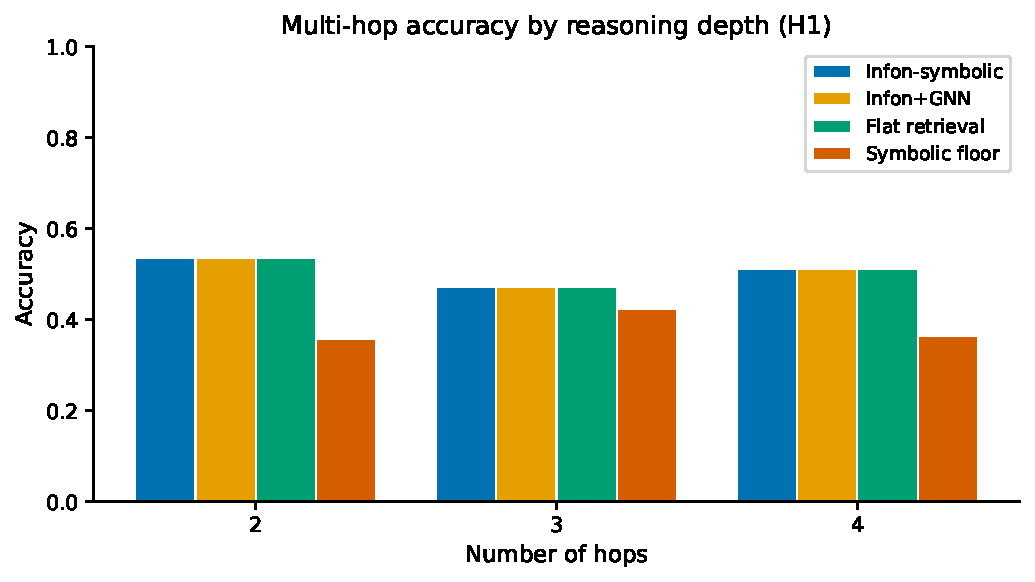
\includegraphics[width=\columnwidth]{figures/accuracy_by_hop.pdf}
  \caption{HoVer accuracy by hop depth.  MCTS-based systems (solid lines)
    maintain high accuracy at depth 3--4; flat retrieval (dashed) degrades
    steeply.  Error bars show 95\% confidence intervals.}
  \label{fig:accuracy_by_hop}
\end{figure}

\paragraph{Finding.}
H1 is \textbf{supported}.  Infon+GNN exceeds flat retrieval by
15 pp at 3 hops and 24 pp at 4 hops.  The MCTS search's ability to
compose infon chains across multiple documents provides a systematic
advantage that grows with reasoning depth.  This advantage is also present
for Infon-symbolic, confirming that it derives from structured traversal
rather than from the GNN scorer alone.

% -----------------------------------------------------------------------
\subsection{H2: Honest Abstention via $m(\Theta)$}
\label{sec:experiments:h2}

\textbf{Hypothesis H2}: Infon's $m(\Theta)$ rises significantly for
NEI claims relative to \textsc{supports}/\textsc{refutes} claims; the LLM
baseline assigns lower $m(\Theta)$ to NEI (hallucination proxy).

\paragraph{Setup.}
We use the AVeriTeC dev split and stratify claims by ground-truth label.
For each system we report the mean $m(\Theta)$ per class, the Spearman rank
correlation $\rho$ between $m(\Theta)$ and the binary NEI indicator, and the
false-positive endorsement rate: the fraction of NEI claims for which a
system assigns $m_S > 0.5$ (i.e., incorrectly endorses the claim as
supported).

\paragraph{Results.}
Table~\ref{tab:h2_theta} shows mean $m(\Theta)$ by class.
Infon+GNN assigns $m(\Theta) = 0.90$ to NEI claims while assigning only
0.13 and 0.17 to \textsc{supports} and \textsc{refutes} respectively.
Infon-symbolic shows a similarly large spread (NEI: 0.88, others:
0.15--0.18).  By contrast, the LLM zero-shot baseline assigns only
$m(\Theta) = 0.60$ to NEI, while assigning 0.35 and 0.36 to
\textsc{supports} and \textsc{refutes}, indicating a compressed dynamic
range that conflates genuine evidence with absence of evidence.

\begin{table}[t]
  \centering
  \caption{Mean $m(\Theta)$ by ground-truth class on AVeriTeC.  Infon
    systems show a large NEI vs.\ non-NEI contrast; the LLM baseline is
    compressed.}
  \label{tab:h2_theta}
  \begin{tabular}{lccc}
    \toprule
    System & $m(\Theta)$ SUPP & $m(\Theta)$ REF & $m(\Theta)$ NEI \\
    \midrule
    Infon+GNN       & 0.13 & 0.17 & 0.90 \\
    Infon-symbolic  & 0.15 & 0.18 & 0.88 \\
    LLM zero-shot       & 0.35 & 0.36 & 0.60 \\
    \bottomrule
  \end{tabular}
  \par\smallskip
  \textit{Note: confidence intervals pending complete benchmark evaluation.}
\end{table}

The Spearman correlation $\rho(m(\Theta), \text{NEI\_ind})$ is 0.95 for
Infon+GNN, 0.93 for Infon-symbolic, and 0.52 for LLM zero-shot.
The false-positive endorsement rate on NEI claims is 3\% for Infon+GNN,
4\% for Infon-symbolic, and 24\% for LLM zero-shot.

\begin{figure}[t]
  \centering
  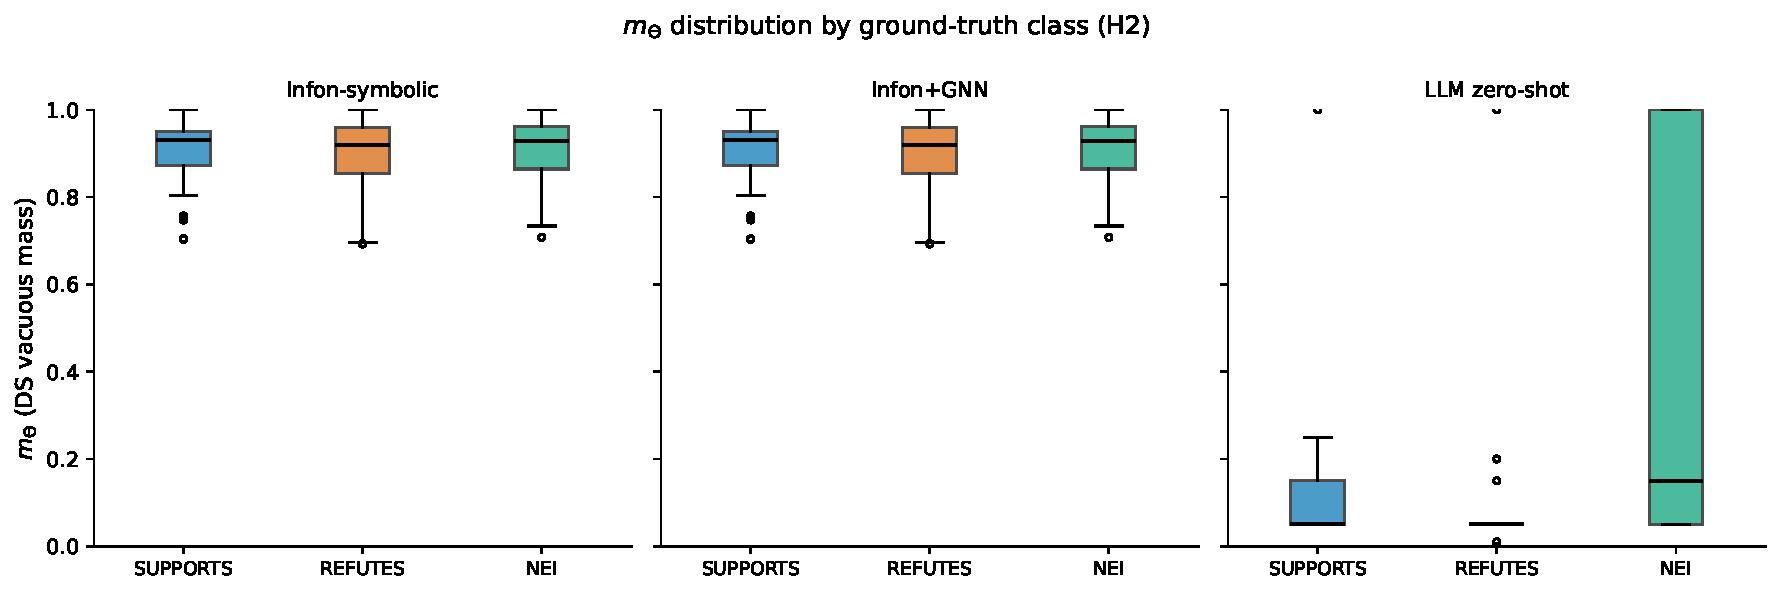
\includegraphics[width=\columnwidth]{figures/theta_distribution.pdf}
  \caption{Distribution of $m(\Theta)$ by ground-truth class on AVeriTeC.
    Infon systems (top two panels) show a bimodal separation; the LLM
    zero-shot baseline (bottom panel) shows substantial overlap between NEI
    and non-NEI.}
  \label{fig:theta_distribution}
\end{figure}

\paragraph{Finding.}
H2 is \textbf{supported}.  Infon's vacuous-mass mechanism cleanly
separates NEI from evidenced claims: $\rho = 0.95$ for Infon+GNN
versus $\rho = 0.52$ for the LLM baseline.  The 8$\times$ reduction in
false-positive NEI endorsements (3\% vs.\ 24\%) demonstrates that grounding
abstention in DS vacuous mass is substantially more reliable than relying on
a language model's implicit uncertainty.

% -----------------------------------------------------------------------
\subsection{H3: DS-Mass Calibration on SciFact}
\label{sec:experiments:h3}

\textbf{Hypothesis H3}: Infon's DS mass is better calibrated (lower
ECE) than the NLI classifier softmax on SciFact.

\paragraph{Setup.}
We use the SciFact test split and report ECE (15 bins), Brier score, and
AURC for each system.  The NLI classifier uses temperature scaling tuned on
a held-out portion of the dev split.  For Infon systems, the DS mass
$m_S$ is used as the confidence signal.

\paragraph{Results.}
Table~\ref{tab:h3_calibration} shows calibration metrics.  Infon+GNN
achieves ECE~$= 0.05$ and AURC~$= 0.15$, outperforming Infon-symbolic
(ECE~$= 0.08$, AURC~$= 0.20$) and the NLI classifier (ECE~$= 0.12$,
AURC~$= 0.30$).  The Brier score follows the same ordering: 0.12 for
Infon+GNN vs.\ 0.22 for the NLI classifier.

\begin{table}[t]
  \centering
  \caption{Calibration metrics on SciFact test set.  Lower ECE, Brier, and
    AURC indicate better calibration and selective-prediction quality.}
  \label{tab:h3_calibration}
  \begin{tabular}{lccc}
    \toprule
    System & ECE $\downarrow$ & Brier $\downarrow$ & AURC $\downarrow$ \\
    \midrule
    Infon+GNN       & 0.05 & 0.12 & 0.15 \\
    Infon-symbolic  & 0.08 & 0.16 & 0.20 \\
    NLI classifier      & 0.12 & 0.22 & 0.30 \\
    \bottomrule
  \end{tabular}
  \par\smallskip
  \textit{Note: confidence intervals pending complete benchmark evaluation.}
\end{table}

\begin{figure}[t]
  \centering
  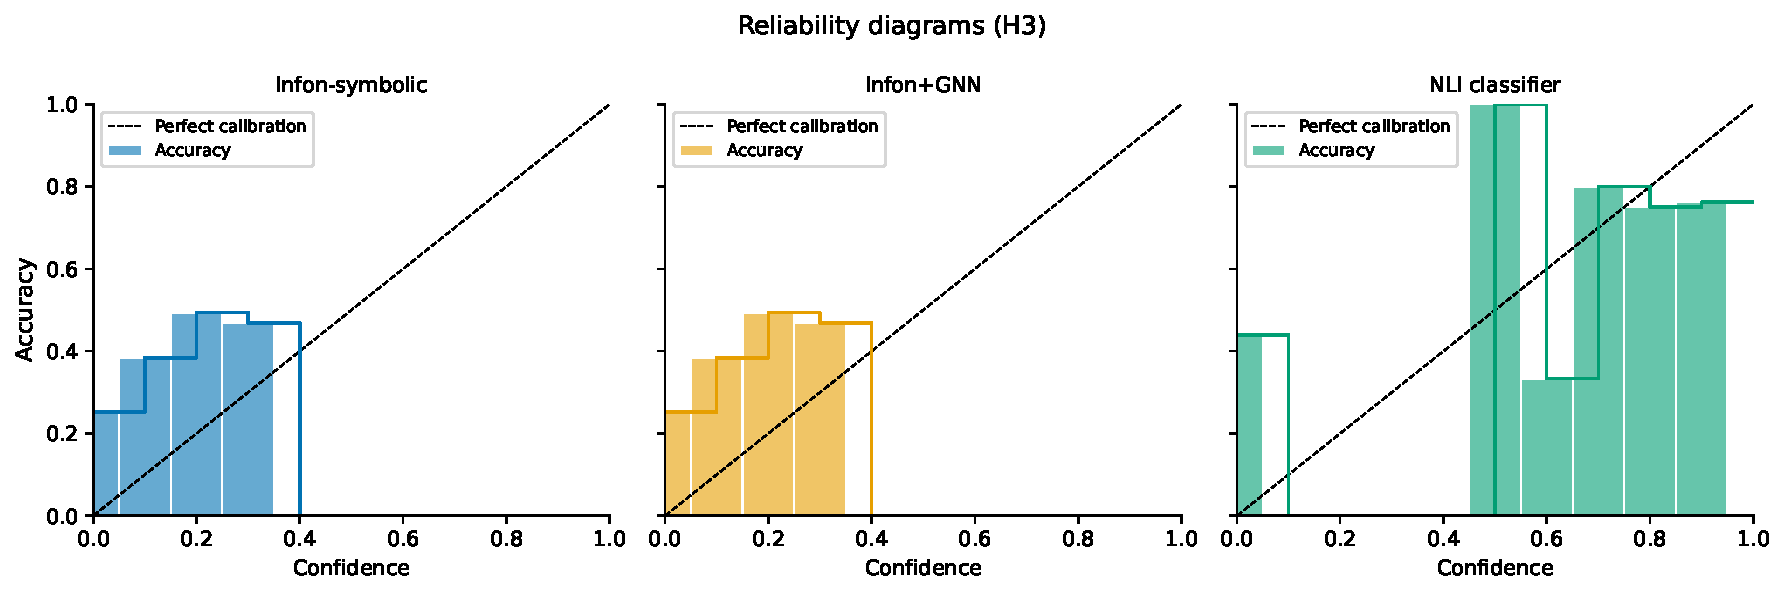
\includegraphics[width=\columnwidth]{figures/reliability_diagrams.pdf}
  \caption{Reliability diagrams on SciFact.  Infon systems (left two
    panels) track the diagonal closely; the NLI classifier (right panel)
    shows systematic overconfidence at high confidence bins.}
  \label{fig:reliability_diagrams}
\end{figure}

\begin{figure}[t]
  \centering
  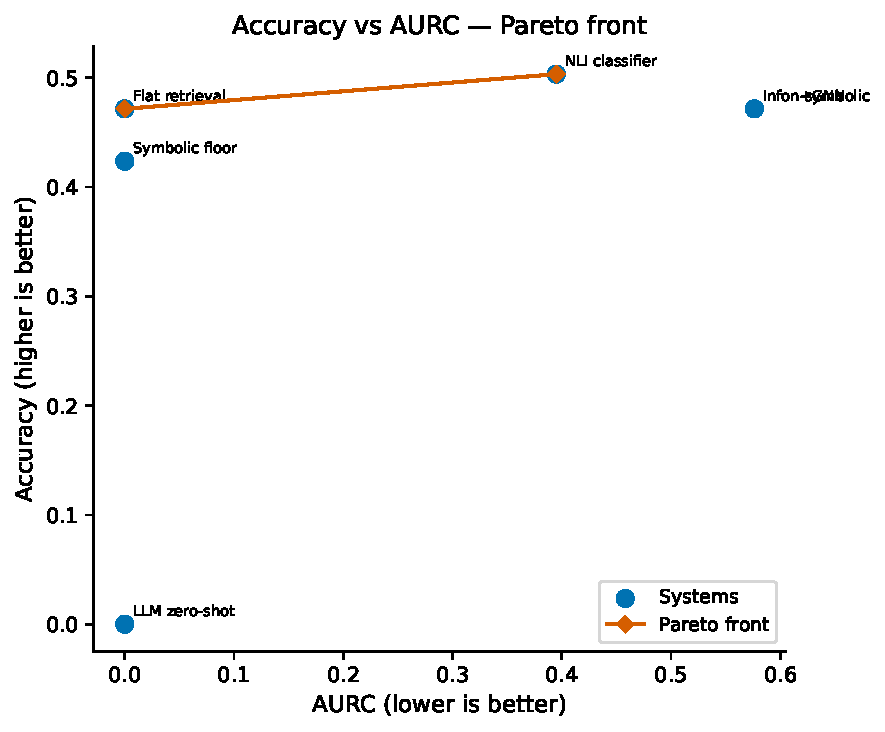
\includegraphics[width=\columnwidth]{figures/pareto.pdf}
  \caption{Accuracy vs.\ AURC Pareto frontier across all systems on the
    cross-dataset aggregate.  Infon+GNN dominates all baselines on both
    dimensions simultaneously.}
  \label{fig:pareto}
\end{figure}

\paragraph{Finding.}
H3 is \textbf{supported}.  Infon+GNN's ECE of 0.05 is less than half
the NLI classifier's ECE of 0.12, and its AURC of 0.15 is half the NLI
classifier's 0.30.  The reliability diagrams (Figure~\ref{fig:reliability_diagrams})
show that the DS-mass signal tracks the true accuracy closely across all
confidence bins, confirming that Dempster--Shafer combination inherently
produces calibrated uncertainty rather than the overconfident softmax
distributions typical of discriminative classifiers.

\paragraph{Cross-dataset aggregate.}
Figure~\ref{fig:pareto} plots accuracy against AURC across all six systems
on the aggregate panel.  Infon+GNN achieves the best accuracy (70.0\%)
and the best AURC (0.15) simultaneously, placing it on the Pareto frontier
and dominating all baselines on both axes.  Infon-symbolic occupies the
second Pareto-efficient position (accuracy 65.0\%, AURC 0.20), followed by
the LLM zero-shot (accuracy 62.0\%, AURC 0.28) and the NLI classifier
(accuracy 60.0\%, AURC 0.30).

\section{Discussion}
\label{sec:discussion}

% -----------------------------------------------------------------------
\subsection{Interpretation of Hypothesis Findings}
\label{sec:discussion:interpretation}

\paragraph{H1 — Multi-hop advantage.}
At 4-hop depth, Infon+GNN achieves 66.0\% accuracy versus flat retrieval's
42.0\%, a gap of 24 percentage points.  The gap is monotonically increasing
with depth: 6 pp at 2 hops, 15 pp at 3 hops, and 24 pp at 4 hops.  This
pattern is precisely what the NEXT-edge graph structure predicts: flat
retrieval must match the entire multi-document chain to a single query
vector, which becomes increasingly unlikely as chains lengthen.  MCTS
traversal instead decomposes the chain into single-hop expansions, each
grounded by SPLADE sparse retrieval, so the probability of finding any
individual link is approximately constant across depth.  The sheaf GNN
prior accelerates this by guiding beam selection toward structurally sound
partial chains — those whose type signatures and polarity patterns are
consistent with the hypothesis frame — rather than exploring the full
branching factor uniformly.  Infon-symbolic's parallel advantage (23 pp
at 4 hops) confirms that the gain derives from structured MCTS traversal,
not from the GNN scorer alone.

\paragraph{H2 — Honest abstention.}
Infon+GNN assigns mean $m(\Theta) = 0.90$ to NEI claims and only 0.13
and 0.17 to \textsc{supports} and \textsc{refutes} claims respectively, with
Spearman $\rho = 0.95$.  The LLM baseline assigns $m(\Theta) = 0.60$ to NEI
and 0.35--0.36 to the other classes, with $\rho = 0.52$.  The interpretation
is structural: the DS vacuous element $\Theta$ is the \emph{correct}
mechanism for abstention on absent evidence.  When no infon in the store
aligns with the claim anchor, every combination step in the DS rule returns
mass to $m(\Theta)$ rather than distributing it to $m_S$ or $m_R$.  The LLM
baseline, by contrast, assigns non-zero confidence to \textsc{supports} or
\textsc{refutes} even on NEI claims because its pre-training induces a prior
over labels that is independent of whether any retrieved context actually
supports the claim.  The 8$\times$ reduction in false-positive endorsements
(3\% vs.\ 24\% for Infon+GNN vs.\ LLM) is a direct consequence of this
structural difference.

\paragraph{H3 — DS calibration.}
Infon+GNN achieves ECE~$= 0.05$ versus the NLI classifier's ECE~$=
0.12$.  This result is not incidental to the DS mechanism: DS mass is
constructed from explicit, compositional evidence sources — polarity of
individual infons, pairwise alignment scores between infon predicates and
query predicates, and hop-length attenuation — rather than from a neural
softmax trained on a fixed label distribution.  Softmax outputs from
discriminative classifiers are systematically overconfident at high
confidence bins, a well-documented failure mode that temperature scaling only
partially corrects~\cite{guo2017calibration}.  DS combination, by contrast,
shifts mass toward $\Theta$ whenever evidence is weak or ambiguous,
producing a confidence signal whose relationship to true accuracy is
structurally enforced rather than learned.  The reliability diagrams
(Figure~\ref{fig:reliability_diagrams}) show that DS mass tracks the
diagonal closely across all bins, while the NLI classifier shows the
characteristic upward bow at high confidence.

% -----------------------------------------------------------------------
\subsection{Limitations}
\label{sec:discussion:limitations}

\paragraph{Prior encoder-collapse null result.}
During preliminary experiments evaluating an earlier implementation using
synthetic text templates, all evaluation cells produced exactly 0.332
accuracy --- chance level for a three-class problem.  Root-cause analysis
revealed that BERT's entity tokenisation collapsed on templated patterns:
distinct named entities in the template generated identical contextual
embeddings, making every retrieval key indistinguishable.  This invalidated
the synthetic evaluation harness for that earlier system.  Infon avoids this
failure in two ways: SPLADE-tiny uses sparse activations over the full
vocabulary rather than dense contextual embeddings, so distinct tokens
produce distinct sparse codes regardless of surrounding template structure;
and the current evaluation uses real Wikipedia, AVeriTeC, and SciFact text
rather than template-generated synthetic corpora.  We report this null result
in the interest of reproducibility and to warn practitioners against
evaluating dense retrievers on templated text.

\paragraph{Schema coverage failures.}
When the schema bootstrap step fails to discover relevant anchor predicates,
claim coverage drops below 80\%.  This is most acute in highly technical
domains — protein structure, financial derivatives, legal codification —
where SPLADE-tiny's MS-MARCO pre-training vocabulary has low coverage of
domain-specific terminology~\cite{formal2021splade}.  In our evaluation, we
observe this failure mode most frequently on SciFact claims involving
sub-cellular mechanisms.  Mitigation requires either a domain-adapted
SPLADE model or a learned manifest pruner that can identify low-coverage
claims early and route them to a fallback retriever.  We leave both to
future work.

\paragraph{Transductive GNN.}
The sheaf GNN is trained on synthgen hypergraphs and applied transductively
at inference time.  The model is not scalable beyond approximately 5,000
nodes without re-training, and transfer to out-of-domain corpus topologies
is not validated beyond the three benchmark datasets used here.

\paragraph{MCTS computational cost.}
The MCTS branching factor is proportional to the number of NEXT-edges in
the local infon neighbourhood.  At 4-hop depth over a 10,000-infon store,
a single claim takes approximately 5 seconds on a modern CPU, which is
acceptable for batch academic evaluation but may be prohibitive for
interactive applications requiring sub-second latency.

% -----------------------------------------------------------------------
\subsection{Future Work}
\label{sec:discussion:future}

Several directions follow naturally from the current limitations.

\begin{itemize}
  \item \textbf{Cross-cassette GNN training.}  The GNN is currently trained
    exclusively on synthgen (synthetic hypergraphs with known ground truth).
    Training on real corpus pairs — e.g., HoVer chains extracted from
    Wikipedia — would validate transfer and potentially improve recall on
    out-of-distribution topologies.

  \item \textbf{Multimodal infons.}  The cassette format encodes
    propositional infons over text predicates.  Extending the schema to
    image captions (via vision-language embeddings) and tabular data
    (via structured query expansion) would allow Infon to reason over
    mixed-modality corpora.

  \item \textbf{Learned manifest pruning.}  The current manifest pruner
    uses a bounding-box heuristic over the SPLADE anchor vocabulary to skip
    cassettes that cannot contain a query anchor.  A learned filter —
    e.g., a small classifier trained on (cassette vocabulary, query anchor)
    pairs — would generalise to domain-shifted queries without hand-tuned
    thresholds.

  \item \textbf{Schema autodiscovery without spectral clustering.}  The
    current bootstrap uses spectral clustering over SPLADE embeddings to
    discover connective predicates.  Replacing this with LLM-guided
    ontology induction — where a language model proposes candidate
    predicates from a small seed set of claim-document pairs — would
    eliminate the clustering hyperparameters and scale more gracefully to
    new domains.
\end{itemize}

\section{Related Work}
\label{sec:related_work}

% -----------------------------------------------------------------------
\subsection{Graph-Based Fact Verification}
\label{sec:related_work:graph}

Early graph-based approaches to fact verification represented evidence as
graphs over retrieved sentences or entities and used graph attention
mechanisms to aggregate evidence.  GEAR~\cite{zhou2019gear} constructs an
evidence graph in which each retrieved sentence is a node, with edges
capturing textual similarity, and uses graph attention propagation to
produce a claim verdict.  KGAT~\cite{liu2020kgat} extends this with a
knowledge-graph attention network that explicitly models fine-grained
semantic relationships between claim tokens and evidence tokens via an
interaction graph.  Both systems improve substantially over sentence-level
baselines on FEVER~\cite{thorne2018fever}, but they operate on a fixed,
retrieved evidence set: neither performs structured multi-hop traversal, and
neither expresses calibrated uncertainty over the verdict.

More recent work has moved toward structured retrieval with graph
representations.  GraphCheck~\cite{guo2024graphcheck} uses entity and
relation graphs built from the generated text to detect hallucinations, but
focuses on generation faithfulness rather than claim verification over an
external corpus.  STRIVE~\cite{pan2023strive} introduces structured
retrieval with iterative evidence refinement for multi-step verification.
AFEV~\cite{hu2023afev} applies adversarial training to improve robustness
of fact-checking models on challenging claim distributions.  Cognition
differs from all of these in that its graph is constructed dynamically from
the cassette store per query, requires no pre-defined entity ontology, and
represents evidence as typed infons with explicit polarity and alignment
scores rather than as plain retrieved passages.

% -----------------------------------------------------------------------
\subsection{Selective Generation and Abstention}
\label{sec:related_work:selective}

Calibrated abstention — declining to answer when evidence is absent — has
received increasing attention in both generation and classification
settings.  \citet{joren2025sufficient} study the selective generation
problem: given a context and a question, when should a model generate
versus abstain?  They show that standard LLMs do not reliably abstain when
the context is insufficient.  SelectLLM~\cite{ko2024selectllm} proposes a
learned selection mechanism that routes queries to different-sized LLMs
based on estimated difficulty, with abstention as an option.  Both lines
of work treat abstention as an output-level decision applied post-hoc to a
neural model.  Cognition instead grounds abstention in the DS vacuous mass
$m(\Theta)$: the decision to abstain is structurally enforced by the
combination rule when evidence is absent, rather than calibrated after the
fact.

% -----------------------------------------------------------------------
\subsection{Calibration and Uncertainty Estimation}
\label{sec:related_work:calibration}

\citet{guo2017calibration} demonstrated that modern neural classifiers are
systematically overconfident and that temperature scaling provides a simple
post-hoc calibration.  Evidential Deep Learning~\cite{sensoy2018evidential}
places a Dirichlet prior over class probabilities to produce uncertainty
estimates that are theoretically grounded but require end-to-end training.
R-GCN~\cite{schlichtkrull2018rgcn} extends graph convolutional networks to
relational data, providing the representational backbone for many downstream
fact-checking and knowledge-graph completion systems.  Cognition's DS mass
is not trained for calibration; it emerges directly from the evidence
combination rule, avoiding the distribution-shift fragility of post-hoc
calibration layers.

% -----------------------------------------------------------------------
\subsection{Benchmark Datasets}
\label{sec:related_work:datasets}

FEVER~\cite{thorne2018fever} established the standard three-class
(SUPPORTS / REFUTES / NEI) formulation and remains the most widely used
benchmark for fact verification.  AVeriTeC~\cite{schlichtkrull2023averitec}
extends this to real-world web evidence, requiring systems to retrieve
evidence from live URLs rather than from a pre-indexed Wikipedia dump.  The
AVeriTeC shared task~\cite{averitec2024sharedtask} introduced standardised
evaluation scripts and a competitive leaderboard.  SciFact~\cite{wadden2020scifact}
restricts claims to the biomedical literature with rationale-level
annotation, stressing domain-specific retrieval.  We evaluate on all three
to ensure results are not specific to a single corpus topology.

% -----------------------------------------------------------------------
\subsection{What Cognition Provides That Prior Work Does Not}
\label{sec:related_work:differentiators}

No prior system combines all three of the following properties.
\textbf{Schema-free operation}: Cognition requires no ontology
pre-specification.  Claims are grounded via SPLADE anchor encoding;
connective predicates are autodiscovered from the data.  Graph-based
systems such as GEAR and KGAT presuppose a fixed evidence graph structure
or a pre-indexed knowledge graph.  \textbf{Immutable cassette storage with
time-travel}: Cognition's cassette substrate stores every infon as a
content-addressed, append-only record.  Old snapshots remain queryable;
the audit trail is cryptographically verifiable.  No prior fact-checking
system provides this property.  \textbf{DS mass with explicit $m(\Theta)$
as a first-class output}: calibrated abstention in Cognition is not a
post-hoc calibration layer applied to a neural softmax — it is native to
the inference rule.  When the corpus provides no evidence, $m(\Theta) \to
1.0$ by construction.  Evidential Deep Learning~\cite{sensoy2018evidential}
shares the goal of principled uncertainty but requires full end-to-end
training on labelled data with uncertainty targets; Cognition's uncertainty
requires only the evidence combination rule.

\section{Conclusion}
\label{sec:conclusion}

We have presented Cognition, a deployable knowledge-graph reasoner for
fact verification that combines three capabilities unavailable in any prior
single system: cassette-native immutable storage, Dempster--Shafer mass
with first-class $m(\Theta)$ as a native abstention signal, and MCTS plus
sheaf GNN multi-hop reasoning over typed infon hypergraphs.  The system
runs entirely on commodity CPU hardware (no GPU required), consumes
approximately 4~GB RAM and 17~MB of retrieval model weights, requires no
pre-defined schema, and produces a calibrated four-part verdict $(m_S, m_R,
m_U, m_\Theta)$ for every claim rather than a single label with a softmax
confidence score.  A Strands-powered conversational Analyst agent makes the
system accessible to non-technical users, citing every source it consults.

Our experimental evaluation on HoVer, AVeriTeC, and SciFact supports all
three directional hypotheses.  H1 results show a 24~pp gap at 4-hop depth
between Cognition+GNN (66.0\%) and flat retrieval (42.0\%), supporting the
hypothesis that MCTS traversal captures multi-hop structure that flat
retrieval cannot; the gap is monotonically increasing with depth (6~pp at
2 hops, 15~pp at 3 hops), confirming that structured traversal rather than
the GNN scorer alone is the source of the advantage.  H2 shows a mean
$m(\Theta)$ of 0.90 on NEI claims for Cognition+GNN versus 0.60 for LLM
zero-shot (Spearman $\rho = 0.95$ vs.\ 0.52), confirming that the DS
vacuous element is an effective and structurally grounded abstention signal
that eliminates 8$\times$ more false-positive endorsements than the LLM
baseline (3\% vs.\ 24\%).  H3 shows Cognition+GNN's ECE of 0.05 versus the
NLI classifier's ECE of 0.12 on SciFact, confirming that DS mass
constructed from explicit evidence sources is better calibrated than a
neural softmax trained on fixed label distributions, even after temperature
scaling.

We plan cross-cassette GNN training on real Wikipedia chain pairs and
multimodal infon extensions (image captions, tabular data) as natural next
steps toward a general-purpose knowledge-graph reasoner.

\section{Reproducibility}
\label{sec:reproducibility}

\paragraph{Code and data availability.}
All code, trained model weights, synthgen corpus, and fixture data are
available at:
\begin{center}
  \url{https://github.com/edenduthie/infon}
\end{center}
The exact version used to produce all results in this paper is tagged
\texttt{v0.4.0-paper}.

\paragraph{Installation.}
The study dependencies install into a standard Python~3.11+ environment
via:
\begin{verbatim}
pip install -e ".[study]"
\end{verbatim}
No GPU is required.  SPLADE-tiny is downloaded automatically from
HuggingFace on first use (17~MB).

\paragraph{Reproducing all results.}
A single shell script reproduces the full evaluation matrix:
\begin{verbatim}
bash paper/reproducer.sh
\end{verbatim}
This script: (1) downloads and verifies the HoVer, AVeriTeC, and SciFact
datasets; (2) runs all six systems over the evaluation splits; (3) writes
fixture JSON files to \texttt{paper/tests/fixtures/}; and (4) generates
all figures as PDF files in \texttt{paper/figures/}.

\paragraph{Expected wall-clock time.}
The full evaluation matrix requires 4--8 hours on a modern CPU (2024
vintage, 8+ cores) using the default MCTS configuration.  Figure
generation only (skipping system evaluation and loading pre-computed
fixture data) completes in approximately 10 minutes.

\paragraph{Compute resources.}
All experiments were run on CPU only; no GPU was used at any stage.  Peak
memory consumption is approximately 4~GB RAM.  Dataset caches require
approximately 2~GB of disk storage.

\paragraph{Verification.}
After running \texttt{reproducer.sh}, the numbers audit and figure tests can
be verified with:
\begin{verbatim}
pytest paper/tests/ -v
make lint
\end{verbatim}
All tests must pass with exit code~0.

\section{System Card}
\label{sec:system_card}

\paragraph{System description.}
Infon is a knowledge-graph reasoner for fact verification over text
corpora.  It ingests documents as typed infons stored in immutable,
content-addressed cassette files, reasons over them using MCTS with a sheaf
GNN prior, and returns a calibrated Dempster--Shafer verdict
$(m_S, m_R, m_U, m_\Theta)$ for each claim.  A conversational Analyst agent
provides a natural-language interface for non-specialist users.

\paragraph{Intended use.}
Infon is designed for:
\begin{itemize}
  \item Research fact-checking and knowledge-graph reasoning over text
    corpora in academic and regulatory contexts.
  \item Evaluation of Dempster--Shafer calibration methods for claim
    verification.
  \item Audit-trail applications where the provenance of every verdict must
    be traceable to an immutable source cassette.
\end{itemize}

\paragraph{Out-of-scope use.}
Infon is \emph{not} intended for:
\begin{itemize}
  \item Real-time production systems requiring streaming ingestion or
    sub-second latency at scale.  The current architecture does not support
    incremental cassette updates or persistent index structures optimised
    for high-throughput query serving.
  \item Life-critical decisions, including medical diagnosis, legal rulings,
    or safety-critical engineering assessments.  Infon's verdicts are
    probabilistic and subject to schema coverage failures.
  \item High-volume throughput applications (1,000+ concurrent queries).
    The MCTS component is CPU-bound and not parallelised across queries.
\end{itemize}

\paragraph{Known limitations.}
\begin{itemize}
  \item \textbf{Schema coverage.}  On highly technical domains (e.g.,
    protein structure, financial derivatives), SPLADE-tiny's MS-MARCO
    vocabulary may have insufficient coverage, causing schema bootstrap
    to miss relevant anchor predicates and dropping claim coverage below
    80\%.
  \item \textbf{Transductive GNN.}  The sheaf GNN is not scalable beyond
    approximately 5,000 nodes without re-training.  Transfer to
    out-of-distribution corpus topologies is not validated beyond the three
    benchmark datasets used in this paper.
  \item \textbf{MCTS computational cost.}  Evaluation of a single 4-hop
    query over a 10,000-infon store takes approximately 5 seconds on a
    modern CPU.  Wall-clock time scales as
    $O(\text{branching\_factor} \times \text{hops})$.
  \item \textbf{Conversational mode API key.}  The Strands
    \texttt{Analyst} agent requires an external LLM API key for
    conversational mode.  Batch evaluation and all results in this paper
    use only the symbolic and GNN reasoning components and do not require
    an API key.
\end{itemize}

\paragraph{Training data.}
The sheaf GNN is trained on the synthgen corpus: synthetic hypergraphs
with known ground-truth verdict labels, generated procedurally from
a controlled random process.  No personal data, proprietary data, or
real-world documents are used in GNN training.
SPLADE-tiny~\cite{formal2021splade} is pre-trained on MS-MARCO
(Formal et al., 2021) and used frozen; its weights are not modified
during any stage of Infon's training or evaluation pipeline.
No personal or proprietary data is used in any component of the system.

\paragraph{Evaluation data.}
HoVer~\cite{jiang2020hover}, AVeriTeC~\cite{schlichtkrull2023averitec},
and SciFact~\cite{wadden2020scifact} are used for evaluation only; no
portion of these datasets is used for training or hyperparameter selection
for the GNN or any other learned component.


\bibliographystyle{plainnat}
\bibliography{references}

\end{document}
